\section{Analysis}
\label{sec:Analysis}

Before working with the actual data, a simulation sample is used to familiarize oneself with the structure of the data. This simulation sample includes only $B^\pm$ candidates decaying into three Kaons. The distributions of the momenta belonging to the first Kaon is shown in \autoref{fig:momentum}. 

\begin{figure}
	\centering
	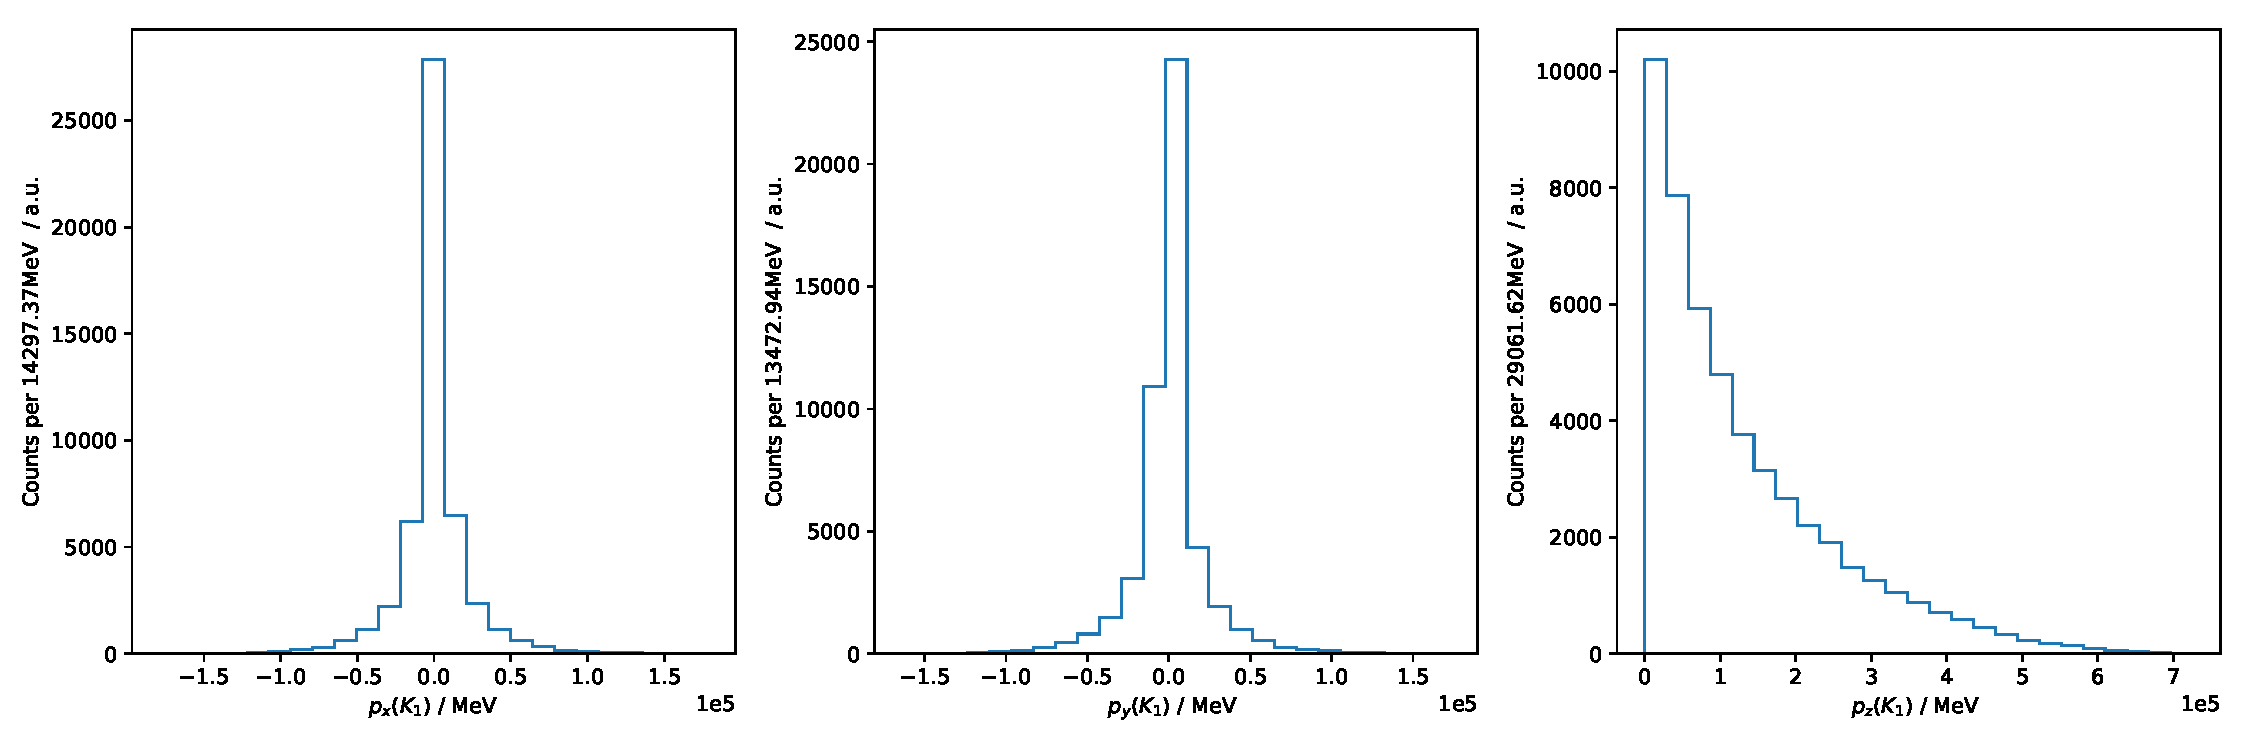
\includegraphics[width=0.9\linewidth]{content/pictures/image_fin/momentum}
	\caption{Momentum distributions of the fist Kaon.}
	\label{fig:momentum}
\end{figure}


From the momenta and the nominal mass of the Kaon $m(K^\pm) = \qty{493.677 \pm 0.015}{\mega\eV }$  the energy carried by the Kaon is determined \cite{pdg}. The Energy distribution is shown in \autoref{fig:energyk1}

\begin{figure}
	\centering
	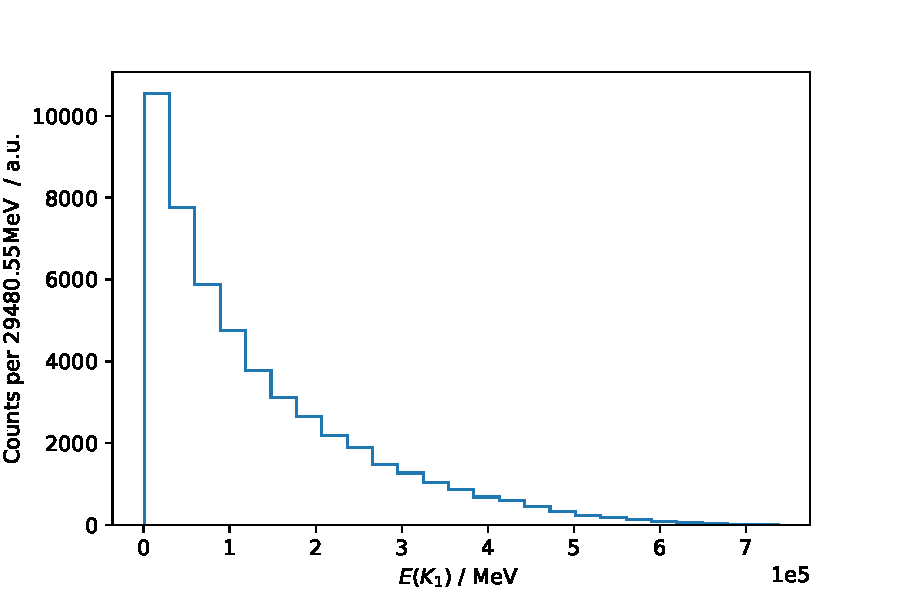
\includegraphics[width=0.6\linewidth]{content/pictures/image_fin/energyK1}
	\caption{Histogram of the energy determined form the fist Kaons momenta.}
	\label{fig:energyk1}
\end{figure}


Using the determined energy and momenta of the Kaons the four momenta of the $B^\pm$ can be calculated. The four moment are then used to determine the invariant mass of the $B^\pm$. This distribution is not shown as the peak around the nominal mass $m(B^\pm) = \qty{5279.41\pm0.07}{\mega\eV}$ is to narrow for histogramming \cite{pdg}. \\


Before working with the data sample an additional requirement is placed on the \texttt{prob} variables to ensure the studied candidates are originating from the $B^\pm \rightarrow K^+ K^- K^\pm$ decay. This requirement is applied, because the data sample contains candidates form additional decays, e.g. including Pions. The values for the requirement on the candidates determined probability are chosen to be: 
\begin{align}
	\mathtt{H1\_probK} &> 0.5\\
	\mathtt{H1\_probPi} &< 0.5
\end{align}

The same steps explained for the simulation sample are then performed on the data sample in order to obtain the $B$-Mesons invariant mass distribution, shown in \autoref{fig:invmass}. 

\begin{figure}
	\centering
	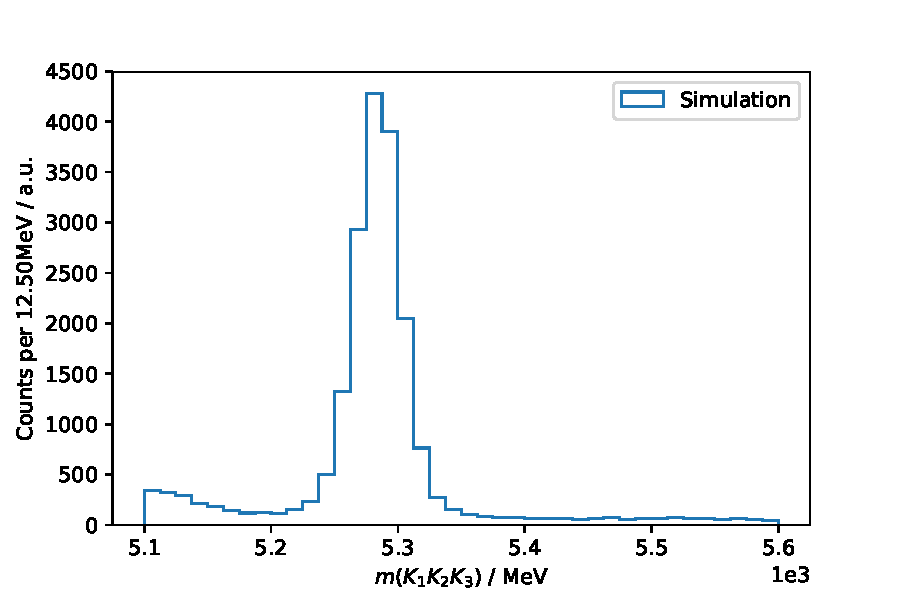
\includegraphics[width=0.6\linewidth]{content/pictures/image_fin/invmass}
	\caption{Invariant mass distribution of the $B^\pm$.}
	\label{fig:invmass}
\end{figure}
In 

In order to calculate the global $CP$-asymmetry $A_\mathrm{CP}$ the signal counts of the $B^+$ and $B^-$ have to be determined. This is achieved by fitting the function 
\begin{equation}
	f(x) = N\exp\left(-\lambda x\right) + A  \exp\left(\frac{(x-\mu)^2}{2\sigma^2}\right)
	\label{eq:fit}
\end{equation} 
onto the counts determined from a histogram and calculating the signal counts as the area under the gaussian function $\sqrt{2\pi}A\sigma$. The plots of the fitted data for both $B^+$ and $B^-$ candidates are given \autoref{fig:fits}


\begin{figure}[H]
	\centering
	\begin{subfigure}{0.45\textwidth}
		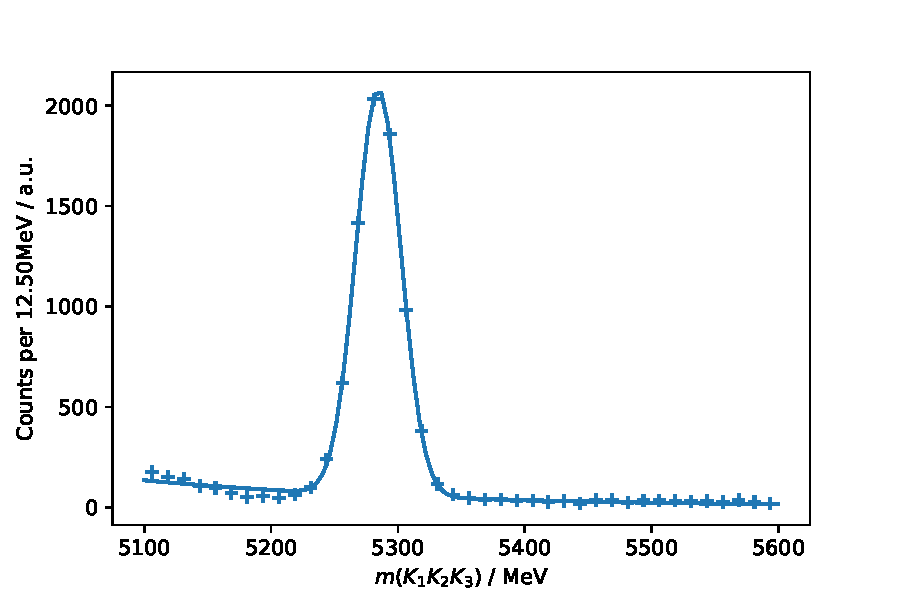
\includegraphics[width=\textwidth]{content/pictures/image_fin/invmassFitBN.pdf}
		\caption{$B^+$}
	\end{subfigure}
	\begin{subfigure}{0.45\textwidth}
		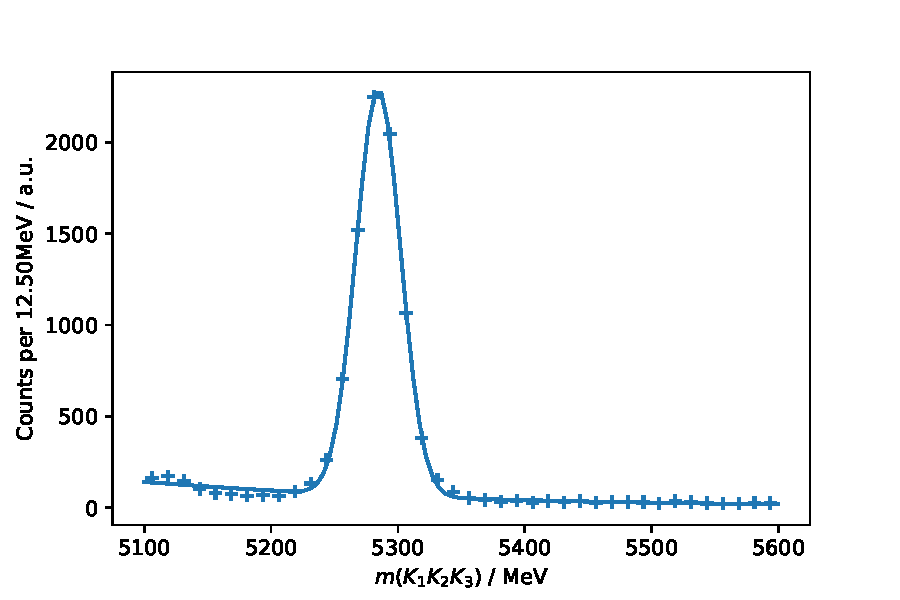
\includegraphics[width=\textwidth]{content/pictures/image_fin/invmassFitBP.pdf}
		\caption{$B^-$}
	\end{subfigure} 
	\caption{Function \autoref{eq:fit} fitted on the counts determined from the histograms of both $B^+$ and $B^-$ candidates.}
	\label{fig:fits}
\end{figure}

The determined signal counts are used to calculate the global asymmetry factor $A_\mathrm{glo}$ using \eqref{eq:asymmetry} and \eqref{eq:A_error}.  The global asymmetry factor calculates to 
\begin{equation}
	A_\mathrm{glo} = \num{0.04469\pm0.00815}
\end{equation}
with a significance of $S = 5.48$. \\

When studying three body decays Dalitz plots are a helpful tool to remove different resonances form the data samples. For the Dalitz plot each possible invariant mass of the combination of two of the three Kaons are created. The two possible resonances, where the sum of the charges is zero are then used to create the Dalitz plot. The Dalitz plots of the simulation sample and the data sample in \autoref{fig:dalitz}.


\begin{figure}[H]
	\centering
	\begin{subfigure}{0.45\textwidth}
		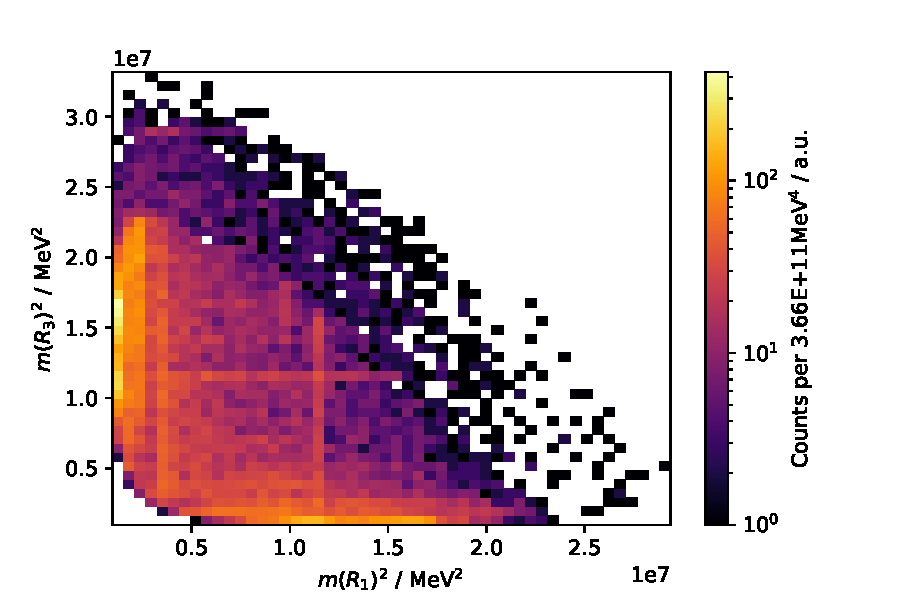
\includegraphics[width=\textwidth]{content/pictures/image_fin/DalitzDataHist.pdf}
		\caption{Data sample}
		\label{subfig:data}
	\end{subfigure}
	\begin{subfigure}{0.45\textwidth}
		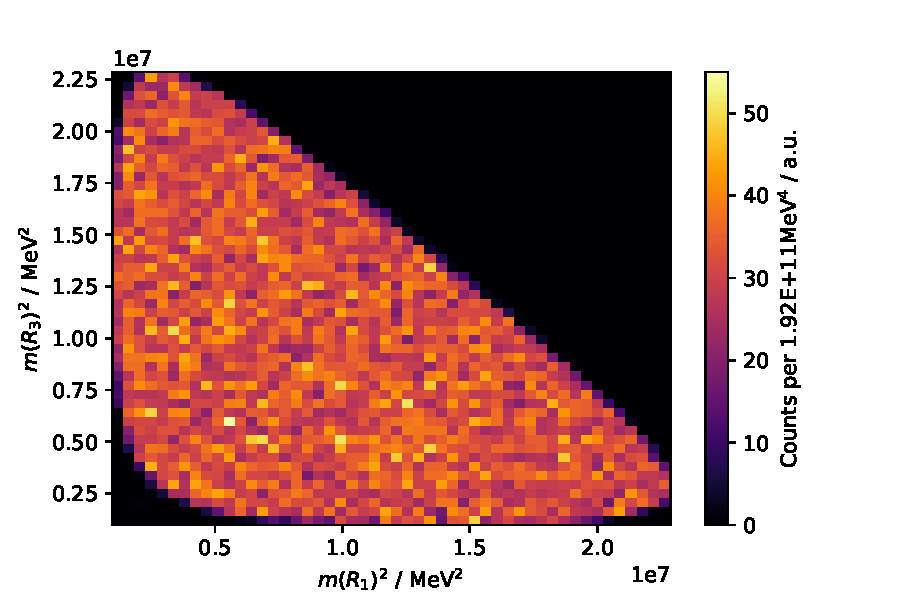
\includegraphics[width=\textwidth]{content/pictures/image_fin/DalitzSimHist.pdf}
		\caption{Simulation sample}
		\label{subfig:sim}
	\end{subfigure} 
	\caption{Dalitz plot of the simulation sample \eqref{subfig:sim} and the data sample \eqref{subfig:data}.}
	\label{fig:dalitz}
\end{figure}

Another way of creating a Dalitz plot is to compare the masses of the resonances and plot the lower mass on one and the higher mass on the other axis, as seen in \autoref{fig:dalitzalt}.

%\begin{figure}
%	\centering
%	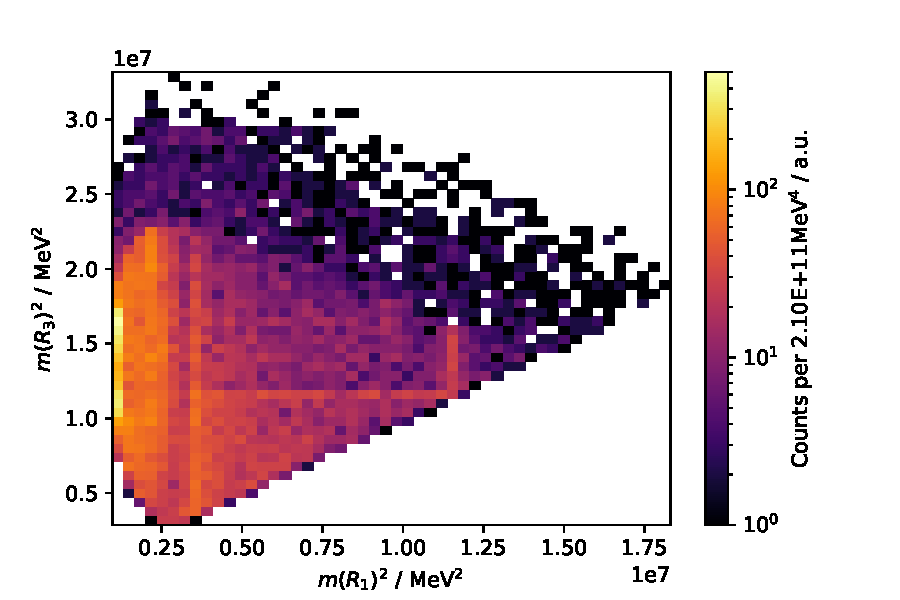
\includegraphics[width=0.6\linewidth]{content/pictures/image_fin/DalitzMINMAXDataHist.pdf}
%	\caption{Alternative Dalitz plot with $R_\mathrm{min}$ and $R_\mathrm{max}$.}
%	\label{fig:dalitzalt}
%\end{figure}

To enhance the plot is created again not as a two dimensional histogram, but as a scatter plot, shown in \autoref{fig:dalitzdata}.

%\begin{figure}
%	\centering
%	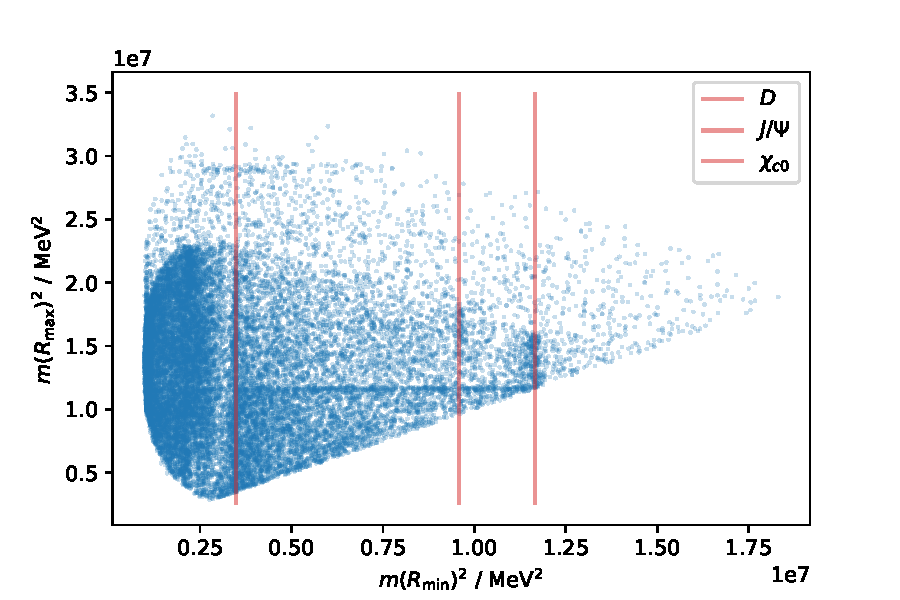
\includegraphics[width=0.6\linewidth]{content/pictures/image_fin/DalitzData}
%	\caption{Scatter plot of the resonance masses squared of the data sample.}
%	\label{fig:dalitzdata}
%\end{figure}

\begin{figure}[H]
	\centering
	\begin{subfigure}{0.45\textwidth}
			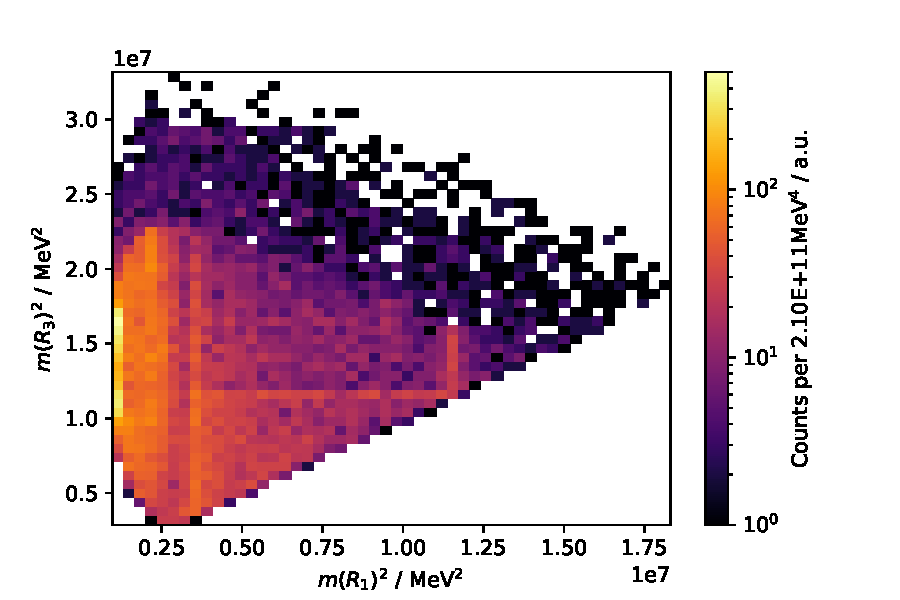
\includegraphics[width=\textwidth]{content/pictures/image_fin/DalitzMINMAXDataHist.pdf}
			\caption{Alternative Dalitz plot with $R_\mathrm{min}$ and $R_\mathrm{max}$.}
			\label{fig:dalitzalt}
	\end{subfigure}
	\begin{subfigure}{0.45\textwidth}
		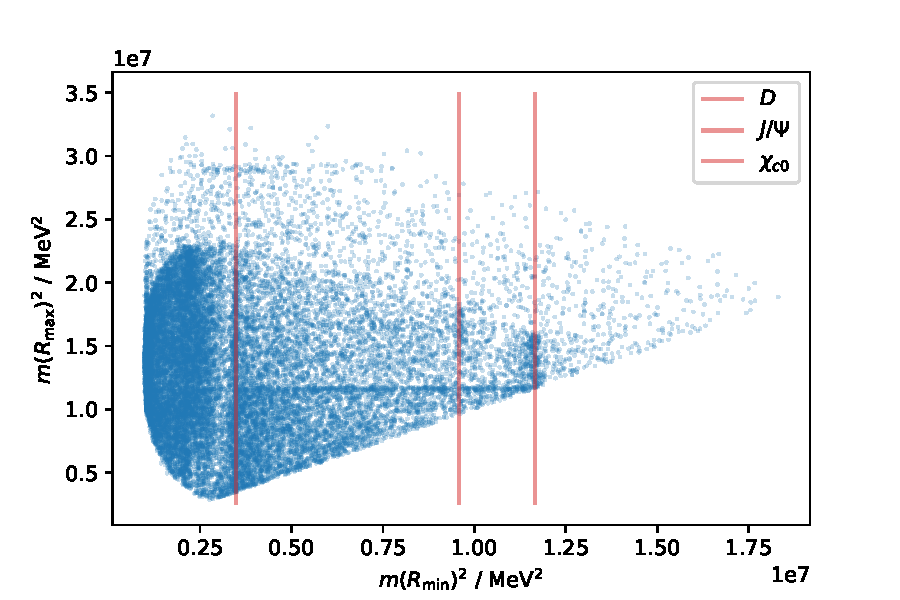
\includegraphics[width=\textwidth]{content/pictures/image_fin/DalitzData}
		\caption{Scatter plot of the resonance masses squared of the data sample.}
		\label{fig:dalitzdata}
	\end{subfigure} 
\end{figure}

In the second plot the resonances can be identified much easier. The unwanted resonances are identified as the $D$-meson, $J\-/\-\psi$ and the $\chi_{c0}$ and then removed by applying another requirement. This requirement is determined by removing the candidates where the $R_1$ and $R_3$ mass are in the range of \qty{20}{\mega\eV} close to the nominal masses of the $D$-meson, $J\-/\-\psi$ or the $\chi_{c0}$.\\

Lastly the local asymmetry is determined. This is achieved by determining the counts in a given energy range. The counts of $B^+$ and $B^-$ are determined respectively by creating two two dimensional histograms, shown in \autoref{fig:dalitzBPM}.

\begin{figure}[H]
	\centering
	\begin{subfigure}{0.45\textwidth}
		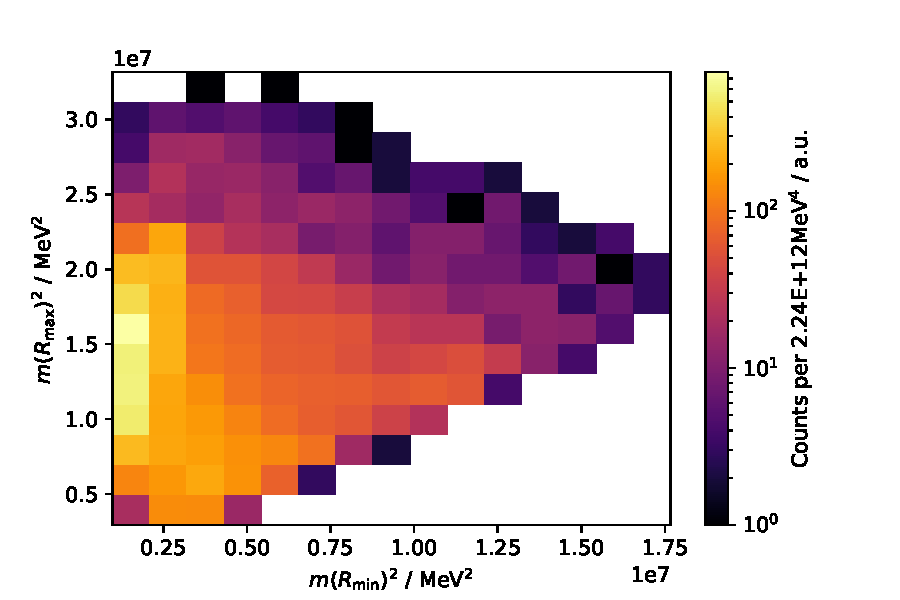
\includegraphics[width=\textwidth]{content/pictures/image_fin/DalitzDataBNhist}
		\caption{$B^-$}
	\end{subfigure}
	\begin{subfigure}{0.45\textwidth}
		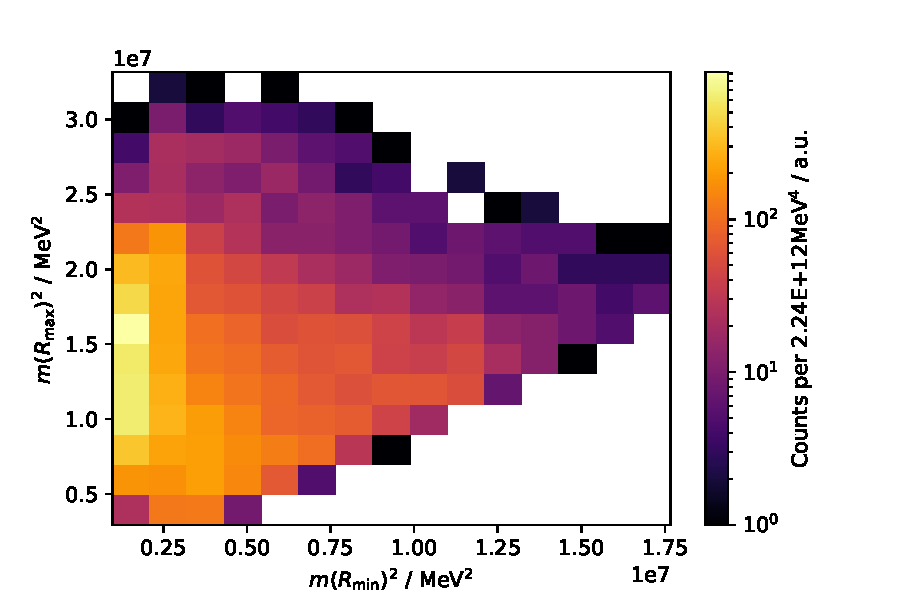
\includegraphics[width=\textwidth]{content/pictures/image_fin/DalitzDataBPhist}
		\caption{$B^+$}
	\end{subfigure} 
	\caption{Two dimensional histograms of the $B^+$ and $B^-$.} 
	\label{fig:dalitzBPM}
\end{figure}

The counts obtained by these plots are used to calculate a "per-bin" asymmetry factor, as seen in \autoref{fig:binA}. Additionally the significance of each bin is determine and shown in \autoref{fig:binAsig}.
 
\begin{figure}[H]
	\centering
	\begin{subfigure}{0.45\textwidth}
		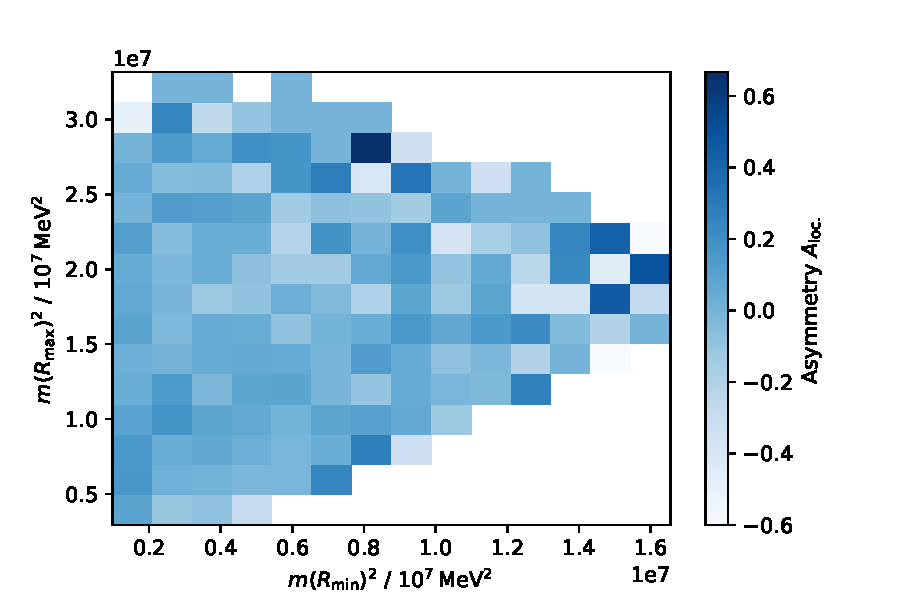
\includegraphics[width=\textwidth]{content/pictures/image_fin/DalitzDataBPhistACPV.pdf}
		\caption{Determined "per-bin"  CP asymmetry factor.}
		\label{fig:binA}
	\end{subfigure}
	\begin{subfigure}{0.45\textwidth}
		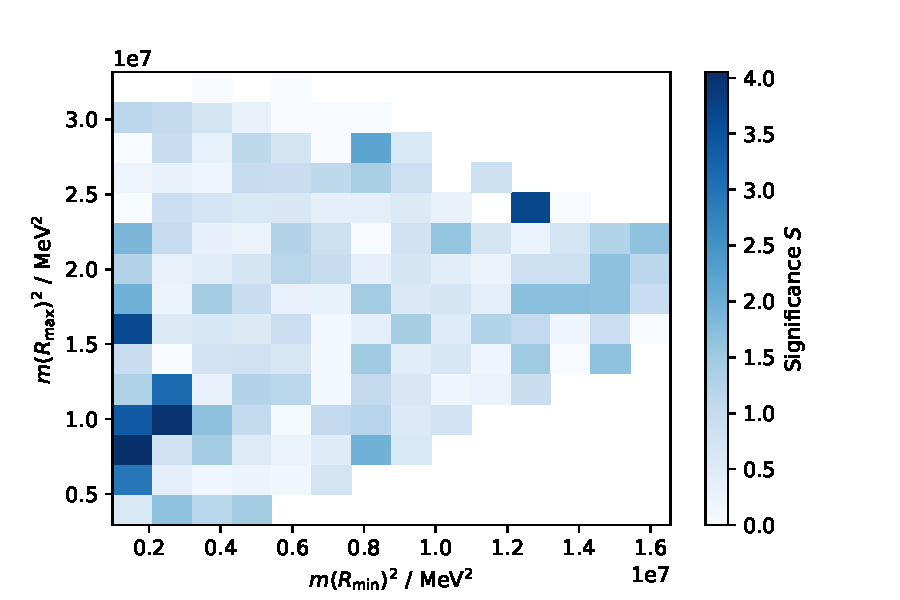
\includegraphics[width=\textwidth]{content/pictures/image_fin/DalitzDataBPhistACPVsig.pdf}
		\caption{Local significance of the calculated CP asymmetry.}
		\label{fig:binAsig}
	\end{subfigure} 
\end{figure}

The region with a high CP asymmetry is chosen as:
\begin{align*}
	\qty{0.98e6}{\mega\eV\tothe{2}} <\ &m(R_\mathrm{max})^2<\qty{4.32e6}{\mega\eV\tothe{2}}\\ \qty{2.92e6}{\mega\eV\tothe{2}} <\ &m(R_\mathrm{min})^2<\qty{21.07e6}{\mega\eV\tothe{2}}
\end{align*}

The candidates in this region are used to determine the CP asymmetry factor via the aforementioned fit method. Additionally the invariant mass distribution of the candidates is histogrammed in \autoref{} to visualize this asymmetry.

\begin{figure}
	\centering
	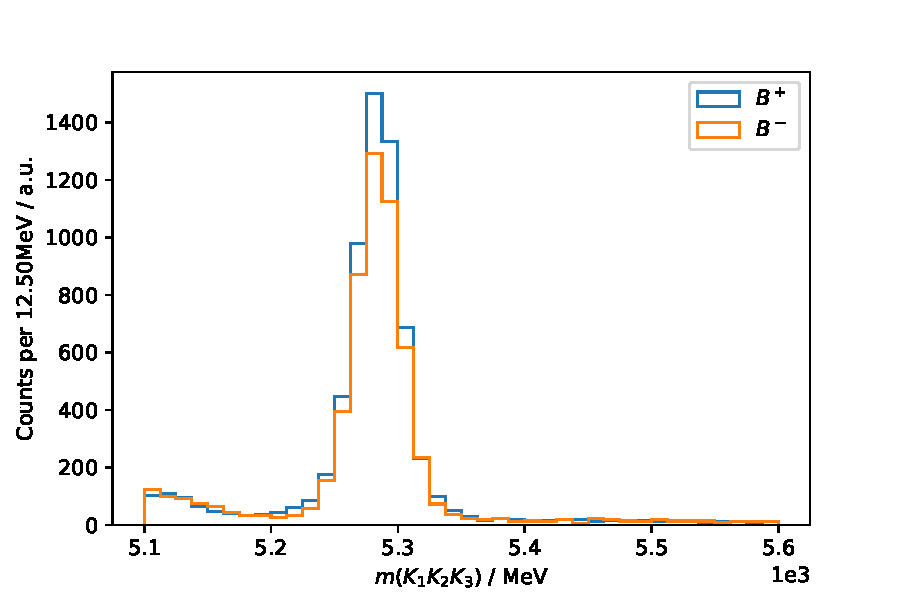
\includegraphics[width=0.6\linewidth]{content/pictures/image_fin/invmassLocAlt}
	\caption{Invariant mass distribution of the $B^+$ and $B^-$ in the high CP asymmetry region.}
	\label{fig:invmasslocalt}
\end{figure}

From the fits mentioned above the local CP asymmetry factor
\begin{equation}
	A_\mathrm{loc} = \num{0.06286\pm0.01017}
\end{equation}
is calculated, with a resulting significance of $S = 6.18$



